\documentclass{ximera}

\addPrintStyle{..}

\begin{document}
	\author{Bart Lambregs}
	\xmtitle{De harmonische oscillator}{}
    \xmsource\xmuitleg


	%% \chapter{Harmonische trillingen}

	Om golven te kunnen beschrijven, behandelen we eerst trillingen. Dat is een iets eenvoudiger verschijnsel. Trillingen zijn heen en weer gaande bewegingen op een lijn. Zo trilt bijvoorbeeld een gitaarsnaar wanneer je hem aanslaat, trilt het rietje in een hobo bij het blazen of trillen elektronen in de antenne van je gsm.
	

	% %%%\section{Enkele voorbeelden}
	% 
	% - geluid
	% - licht
	% - ht is sinus
	

	
	
	%%%\section{De harmonische oscillator}
	
	Als eerste voorbeeld behandelen we een eenvoudig mechanisch systeem: een massa die aan een veer is bevestigd. We noemen dit een massa-veersysteem. En zoals we al zo vaak hebben gedaan, beschouwen we een model waar geen wrijving aanwezig is. Laten we bovendien de veer een horizontale oriëntatie geven zodat we ook de zwaartekracht buiten beschouwing kunnen laten.
	\begin{image}
	
	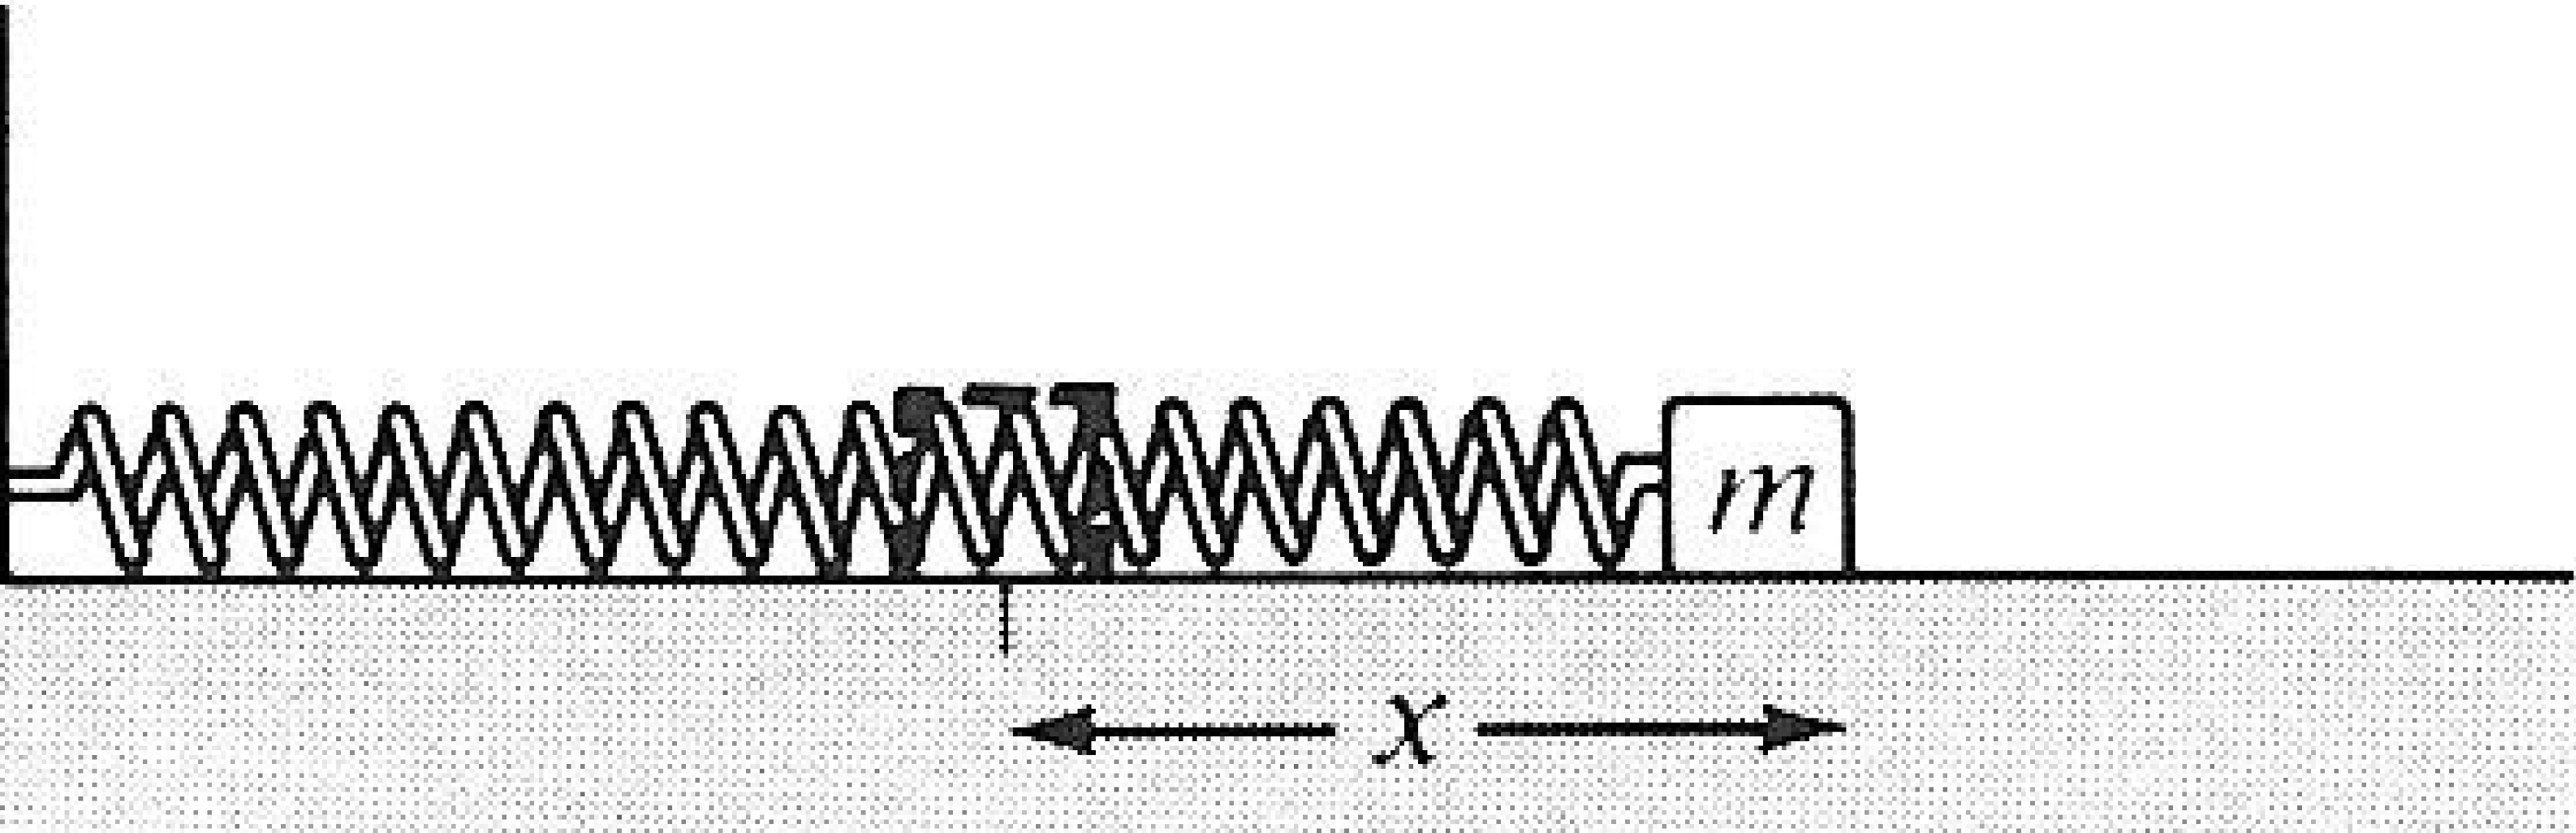
\includegraphics[width=0.8\textwidth]{kogeltegenveer2}
	\end{image}
	Wanneer we de massa uit de positie halen waar de veer zijn rustlengte heeft en hem vervolgens loslaten, voert de massa een trilling uit. We constateren dat hij heen en weer beweegt waarbij hij steeds door de evenwichtspositie gaat. Deze beweging willen we natuurlijk uit onze natuurwetten tevoorschijn zien komen. Meer bepaald moet de tweede wet van Newton -- ons beginsel der beginselen in de klassieke mechanica -- de beweging opleveren. De trilling is een mechanisch verschijnsel en moet dus te verklaren zijn met behulp van die natuurwetten. 
	
	Om de beweging te kunnen vinden, moeten we het systeem vrij maken -- alle krachten erop tekenen. We hebben dus de resulterende kracht nodig. Omdat het lichaam op een ondergrond rust en geen verticale versnelling heeft, heffen de normaalkracht en de zwaartekracht elkaar op. De resulterende kracht is bijgevolg de veerkracht. We gebruiken de wet van Hooke en gieten de component van de kracht volgens de bewegingsrichting in de vorm zoals we ze al kennen:\footnote{Deze beschrijving van de veerkracht is natuurlijk een benadering. Ze is maar geldig voor zolang de veer een niet te grote uitwijking kent. Het minteken zorgt voor een terugroepkracht; wanneer de coördinaat $x$ positief is, is de component van de kracht negatief en wanneer de coördinaat negatief is, is de component positief.}
	\begin{eqnarray*}
	F(x)=-kx
	\end{eqnarray*}
	Nu dat we ons model voor het massa-veersysteem hebben, kunnen we opzoek naar de beweging die de massa uitvoert. Hoe ziet de trilling er precies uit? De tweede wet van Newton dus \ldots
	\begin{eqnarray}
	F&=&ma\nonumber\\
	&\Downarrow&\nonumber\\
	-kx&=&m\frac{d^2x}{dt^2}\nonumber\\
	&\Updownarrow&\nonumber\\
	\frac{d^2x}{dt^2}+\frac{k}{m}x&=&0
	\end{eqnarray}
	\ldots\,en toen kwamen we uit bij een \ldots\,\emph{differentiaalvergelijking}. Om meer precies te zijn: een tweede-orde lineaire differentiaalvergelijking met constante coöefficiënten. Dat klinkt redelijk ingewikkeld. In feite is het ook niet zo simpel. We zijn opzoek naar de beweging, wat betekent dat we de positie $x$ in functie van de tijd willen vinden -- de functie $x(t)$ dus. De vergelijking die we gevonden hebben is niet zozeer een algebra\"ische vergelijking in een onbekende variabele $x$ (zoals bijvoorbeeld een tweedegraadsvergelijking) dan wel \emph{een vergelijking voor een functie}!\footnote{Wanneer we de impliciete afhankelijkheid van de tijd expliciet aangeven,ziet de vergelijking er als volgt uit
	\begin{eqnarray*}
	\frac{d^2x(t)}{dt^2}+\frac{k}{m}x(t)=0
	\end{eqnarray*}} We zoeken dus een functie die aan de vergelijking voldoet. Een functie die voldoet is dan een oplossing van de vergelijking en dus een mogelijke beweging die de massa kan volgen. We spreken hier in eerste instantie over \emph{een} oplossing omdat er a priori\footnote{Vooraf beschouwd. Zonder het gezien, ervaren of onderzocht te hebben.} verschillende oplossingen kunnen zijn.
	
	Het oplossen van differentiaalvergelijkingen is bijna een stiel op zich. Want dergelijke vergelijkingen zijn er in alle maten, geuren, kleuren en vooral moeilijkheidsgraden. En aangezien we die cursus willen overlaten aan degene die zich bij verdere studies hierin wil verdiepen, hebben wij op dit moment geen directe manier om tot de oplossingen te komen. Dat betekent dat we hier iets creatiever zullen moeten zijn en de methode van het ge\"inspireerd gokken zullen moeten toepassen \ldots In de modus van minder hoge ambities, kunnen we in eerste instantie een functie uit onze hoed toveren en nagaan of ze een oplossing is. Dat is natuurlijk onbegonnen werk wanneer we \'alle functies nagaan\footnote{Zoals het ook voor een schaakcomputer onbegonnen werk zou zijn, moest hij alle mogelijke zetten evalueren om de beste er uit te kunnen pikken.} maar haalbaar wanneer we ons fysisch inzicht erbij halen\footnote{Zoals ook een schaker alleen maar die paar zetten bestudeert waarvan hij ziet dat ze de moeite waard zijn.}. Zo moet de functie de beweging beschrijven en zullen de vergelijkingen voor een EVRB naar alle waarschijnlijkheid niet voldoen. De massa gaat heen en weer zodat we met een functie te maken moeten hebben die dat ook doet. Waarom zou dus een \emph{sinusfunctie} niet voldoen \ldots?!
	\begin{image}
	
	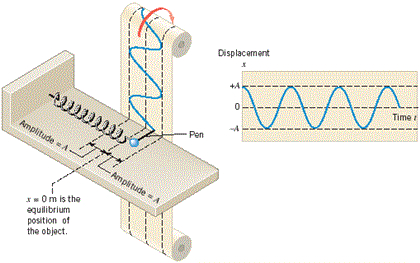
\includegraphics[width=.6\textwidth]{ht_papierrol}
	\end{image}
	
	Om te proberen nemen we een eenvoudige sinusfunctie $x(t)=\sin\omega t$. Bij het invullen in de vergelijking (\ref{diffvgl_ht}) moeten we voor de eerste term in het linkerlid de tweede afgeleide berekenen; $x''(t)=-\omega^2\sin\omega t$. De tweede term geeft bij het invullen $\frac{k}{m}\sin\omega t$. Wil nu de voorgestelde functie een oplossing zijn, dan moet hetgeen we verkregen hebben, gelijk zijn aan het rechterlid -- namelijk nul.
	\begin{eqnarray*}
	 -\omega^2\sin\omega t+\frac{k}{m}\sin\omega t=0\Leftrightarrow\left(-\omega^2+\frac{k}{m}\right)\sin\omega t=0\Leftrightarrow\omega^2=\frac{k}{m}
	\end{eqnarray*}
	In de laatste overgang hebben we gebruik gemaakt van het feit dat de sinus welliswaar nul kan worden maar dit nooit voor \'alle tijdstippen het geval is. De vergelijking moet altijd opgaan -- niet enkel voor een paar momenten in de tijd. Wanneer we dus $\omega=\sqrt{k/m}$ nemen, is de voorgestelde functie een oplossing van de differentiaalvergelijking. We hebben zowaar een mogelijke beweging gevonden die de massa kan uitvoeren!
	
	Natuurlijk hebben we nu slechts \emph{een} oplossing. Misschien zijn er nog. Want, waarom zou een cosinusfunctie niet voldoen? Een cosinusfunctie kunnen we beschrijven als een verschoven sinusfunctie zodat een sinusfunctie in algemene vorm $x(t)=a\sin(b(t-c))+d$ het proberen waard is. We kiezen voor het gemak $d$ gelijk aan nul\footnote{Dit komt overeen met het plaatsen van de oorsprong in de evenwichtspositie van de massa.} en geven in deze context de andere parameters andere symbolen: $a$ vervangen we door $A$, $b$ door $\omega$ en $-bc$ door $\varphi$. Die parameters hebben nl. een iets meer fysische betekenis -- waarover later meer. Ga nu na\footnote{Doe dit effectief. En nee, al liggend in je bed en kijkend naar dit blad voldoet niet aan de imperatief. Iets nagaan in deze exacte wereld van wiskunde en natuurkunde doet men met pen en papier / bord en krijt. Eventueel bijgestaan door een computer.} dat de functie 
	\begin{eqnarray*}
	x(t)=A\sin(\omega t+\varphi)\quad\mathrm{met}\quad\omega=\sqrt{\frac{k}{m}}
	\end{eqnarray*}
	een oplossing is van de differentiaalvergelijking. In feite is dit de algemene oplossing van de differentiaalvergelijking. Hier hebben we de existentie aangetoond; het feit dat er een oplossing bestaat. De uniciteit ervan -- het feit dat er geen andere functie bestaat -- is nog een ander paar mouwen.
	
	Samengevat vinden we dat voor een lineaire terugroepkracht $F=-kx$ de beweging een harmonische trilling is. Ook het omgekeerde is waar: voert een lichaam een harmonische trilling uit, dan is de kracht lineair en steeds naar de oorsprong gericht.
	\begin{eqnarray}
	\frac{d^2x}{dt^2}+\frac{k}{m}x&=&0\nonumber\\
	&\Updownarrow&\nonumber\\
	x(t)=A\sin(\omega t+\varphi)\quad&\mathrm{met}&\quad\omega=\sqrt{\frac{k}{m}}
	\end{eqnarray}
	We hebben nu de wiskundige oplossing van de differentiaalvergelijking gevonden. De massa trilt sinusoöidaal in de tijd. Vandaar dat we over een harmonische trilling spreken.
	
	De verschillende parameters die in de oplossing (\ref{opl_diffvgl_ht}) voorkomen, willen we fysisch kunnen interpreteren. We willen hun betekenis kennen. Het gemakkelijkste is misschien terug te grijpen naar de algemene sinusfunctie. Daar stond de parameter $a$ voor de amplitude. Dat is dus hier voor $A$ niet anders; $A$ stelt de amplitude van de trilling voor. Voor de parameter $b$ hebben we de gelijkheid $b=\frac{2\pi}{p}$ waarin $p$ de periode van de functie is. Omdat onze onafhankelijke variabele de tijd is, is de fysische interpretatie van $p$ de tijd van \'e\'en cyclus -- waarvoor we het symbool $T$ gebruiken. 
	\begin{image}
	
	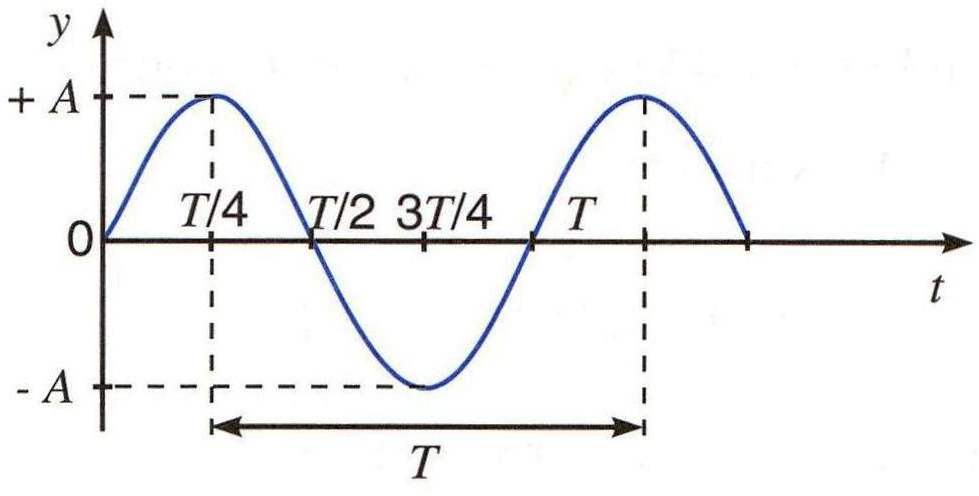
\includegraphics[width=.7\textwidth]{ht_tijd}
	\end{image}
	Voor de parameter $\omega$, die we de pulsatie noemen, geldt dus
	\begin{eqnarray*}
	\omega=\frac{2\pi}{T}
	\end{eqnarray*}
	De pulsatie bepaalt dus de frequentie waarmee de massa trilt. Aangezien voor het massa-veersysteem geldt dat $\omega=\sqrt{k/m}$, kunnen we een uitdrukking voor periode en de frequentie vinden:
	\begin{eqnarray*}
	T=2\pi\sqrt{\frac{m}{k}},\quad f=\frac{1}{2\pi}\sqrt{\frac{k}{m}}
	\end{eqnarray*}
	De frequentie wordt bepaald door de sterkte van de veer en de grootte van de massa. Een grotere massa levert een kleinere frequentie op (de traagheid is groter) en een sterkere veer zorgt voor een grotere frequentie (de massa krijgt een grotere versnelling). De amplitude speelt blijkbaar geen rol.
	
	De parameter $\varphi$ is iets lastiger om inzichtelijk te kunnen duiden. Net zoals de amplitude wordt ze bepaald door de \emph{beginvoorwaarden}. Zo is de amplitude afhankelijk van bijvoorbeeld de afstand uit de evenwichtspositie waarop we de massa vanuit rust loslaten of van de snelheid die we ze bij initiatie van de beweging meegeven. De parameter $\varphi$ wordt bepaald door de positie van de massa op het tijdstip $t=0$. Immers is $x_0=x(t=0)=A\sin(\varphi)$. Het argument van de sinus\footnote{Het argument van de sinus is hetgeen waarvan de sinus wordt genomen/hetgeen dat tussen haakjes staat.} $\omega t+\varphi$ noemen we ook wel de \emph{fase} van de trilling zodat $\varphi$ de \emph{beginfase} wordt genoemd. De fase drukken we natuurlijk uit in radialen. De fase bepaalt waar we ons in de cyclus bevinden. 
	%\begin{image}
	%
	%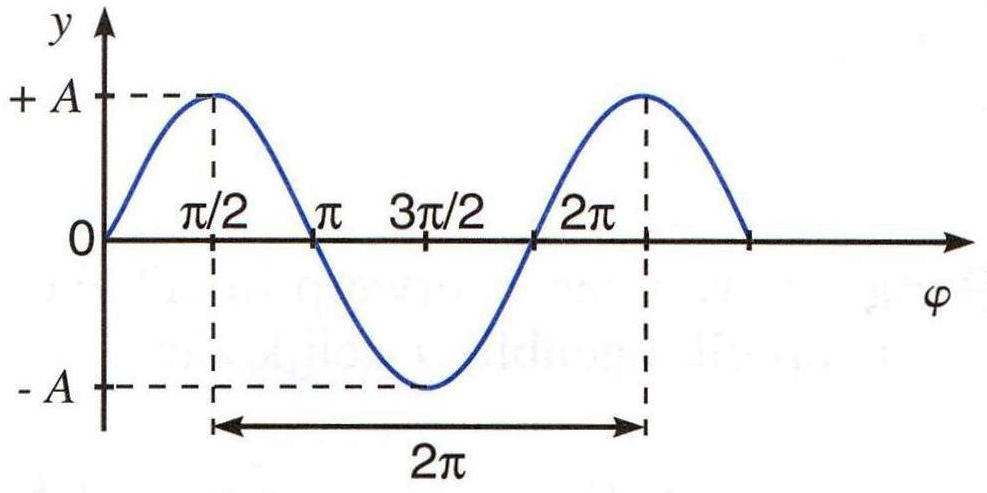
\includegraphics[width=.7\textwidth]{ht_fase}
	%\end{image}
	%%%%\newline
	De beginfase bepaalt dan ook de beginpositie. Zo is bijvoorbeeld de functie maximaal wanneer het argument $\pi/2$ is, wat betekent dat de massa op haar maximale uitwijking is. Is dus de beginfase gelijk aan $\pi/2$, dan begint de trilling vanuit haar maximale uitwijking. Een beginfase van $3\pi/2$ komt overeen met een minimale waarde bij het begin. In figuur \ref{beginposbeginfase} zie je verschillende mogelijkheden voor de beginfase, hier weergegeven als $\varphi_0$.
	
	Nu dat we de positie in functie van de tijd kennen, vinden we door af te leiden de snelheid en de versnelling van de massa. 
	\begin{eqnarray*}
	x&=&A\sin(\omega t+\varphi)\\[3mm]
	v=\frac{dx}{dt}&=&\omega A\cos(\omega t+\varphi)\\[3mm]
	a=\frac{d^2x}{dt^2}&=&-\omega^2A\sin(\omega t+\varphi)=-\omega^2x
	\end{eqnarray*}
	Merk op dat de versnelling op een constante ($\omega^2$) na tegengesteld is aan de positie. Dat is niet verwonderlijk aangezien we te maken hebben met de wet van Hooke en volgens de tweede wet van Newton de versnelling recht evenredig is met de kracht. 
	
	%%\newpage
	
	\begin{image}
		
		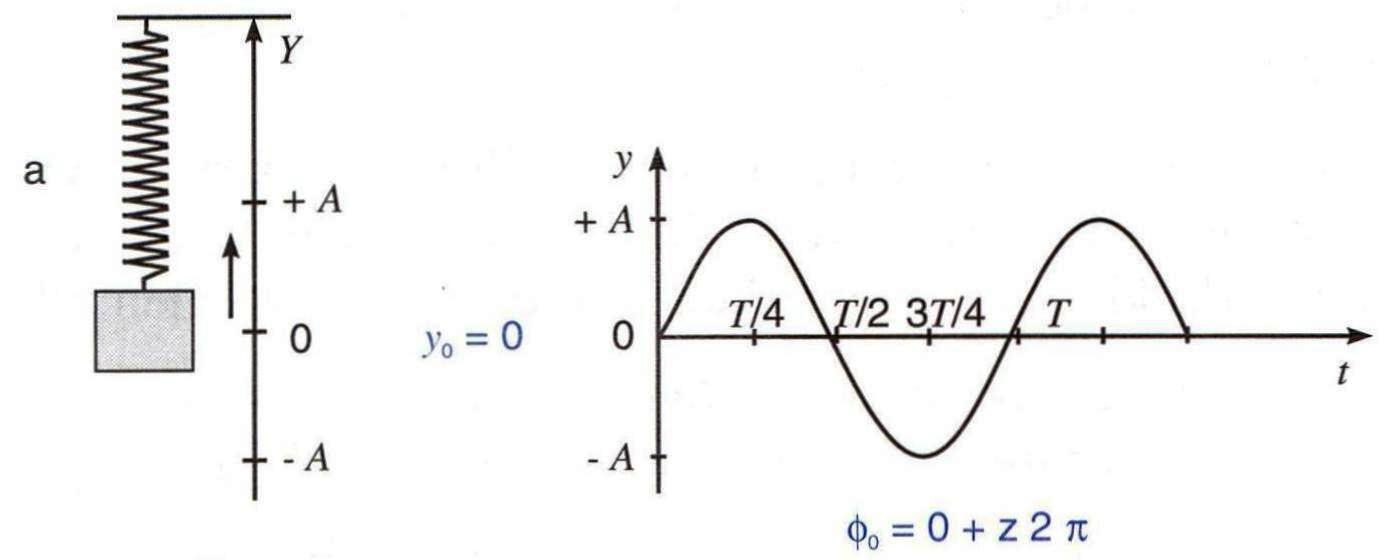
\includegraphics[width=.9\textwidth]{trillendeveer_a}
		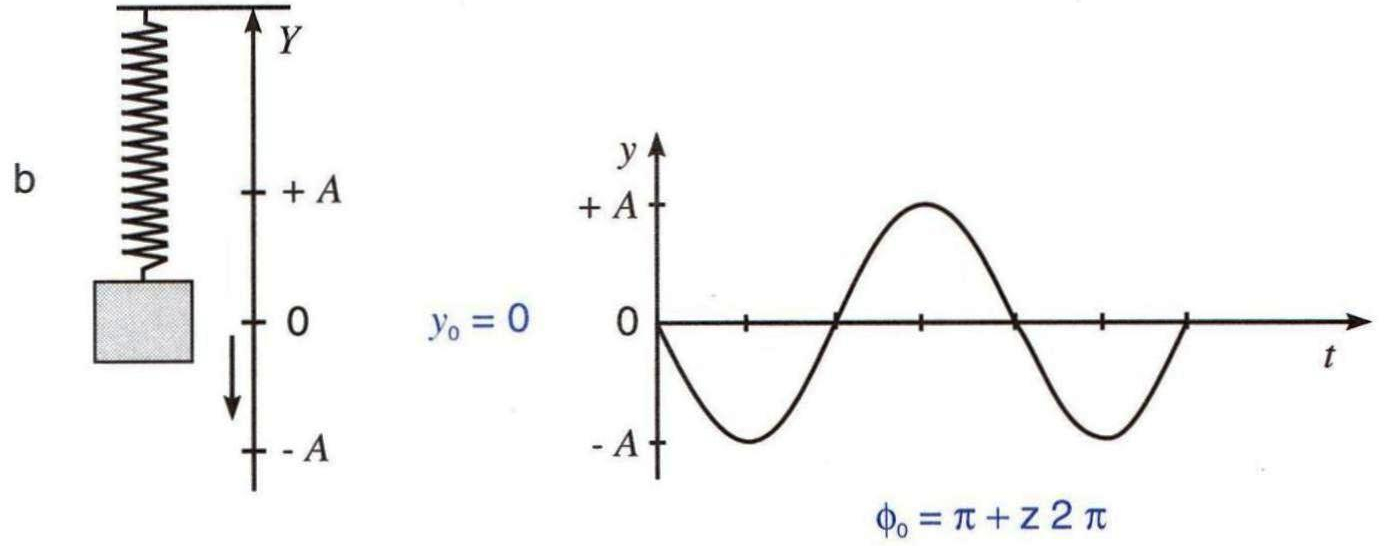
\includegraphics[width=.9\textwidth]{trillendeveer_b}
		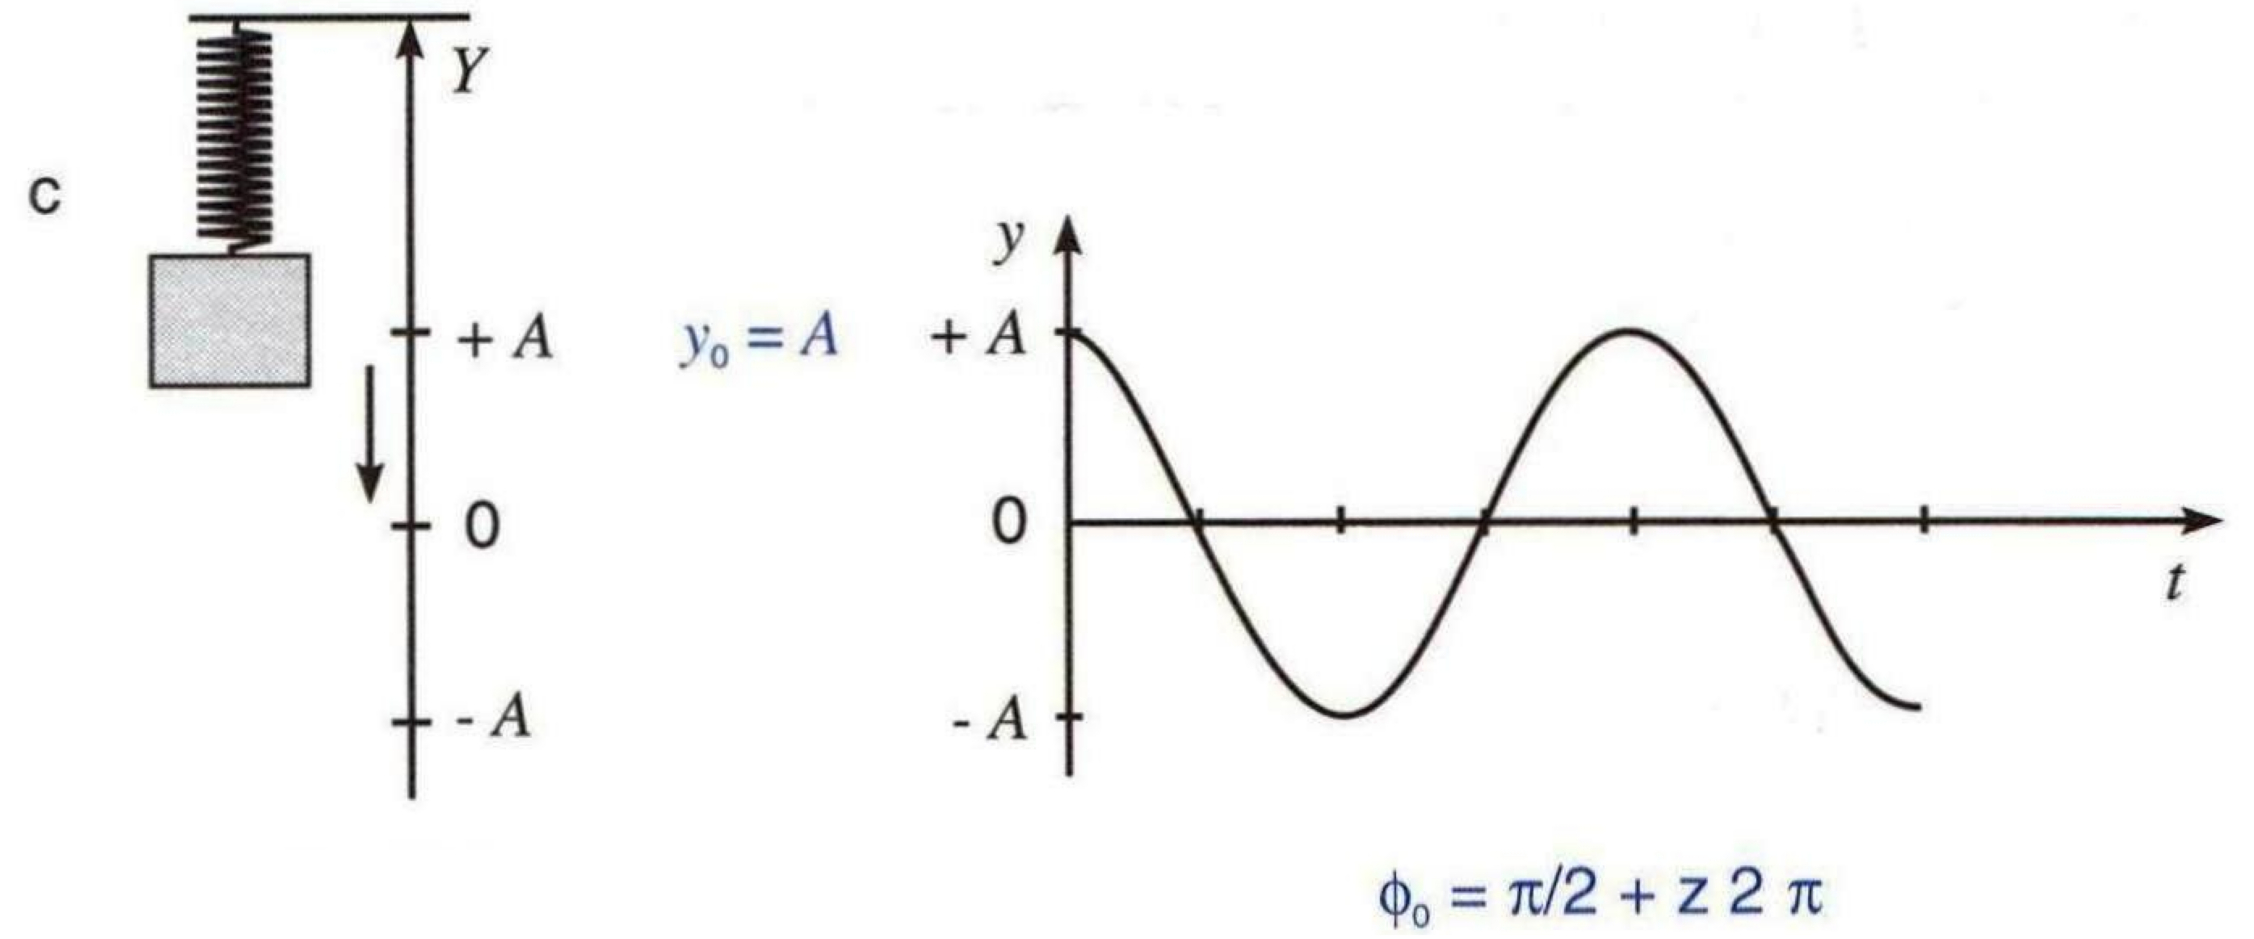
\includegraphics[width=.9\textwidth]{trillendeveer_c}
		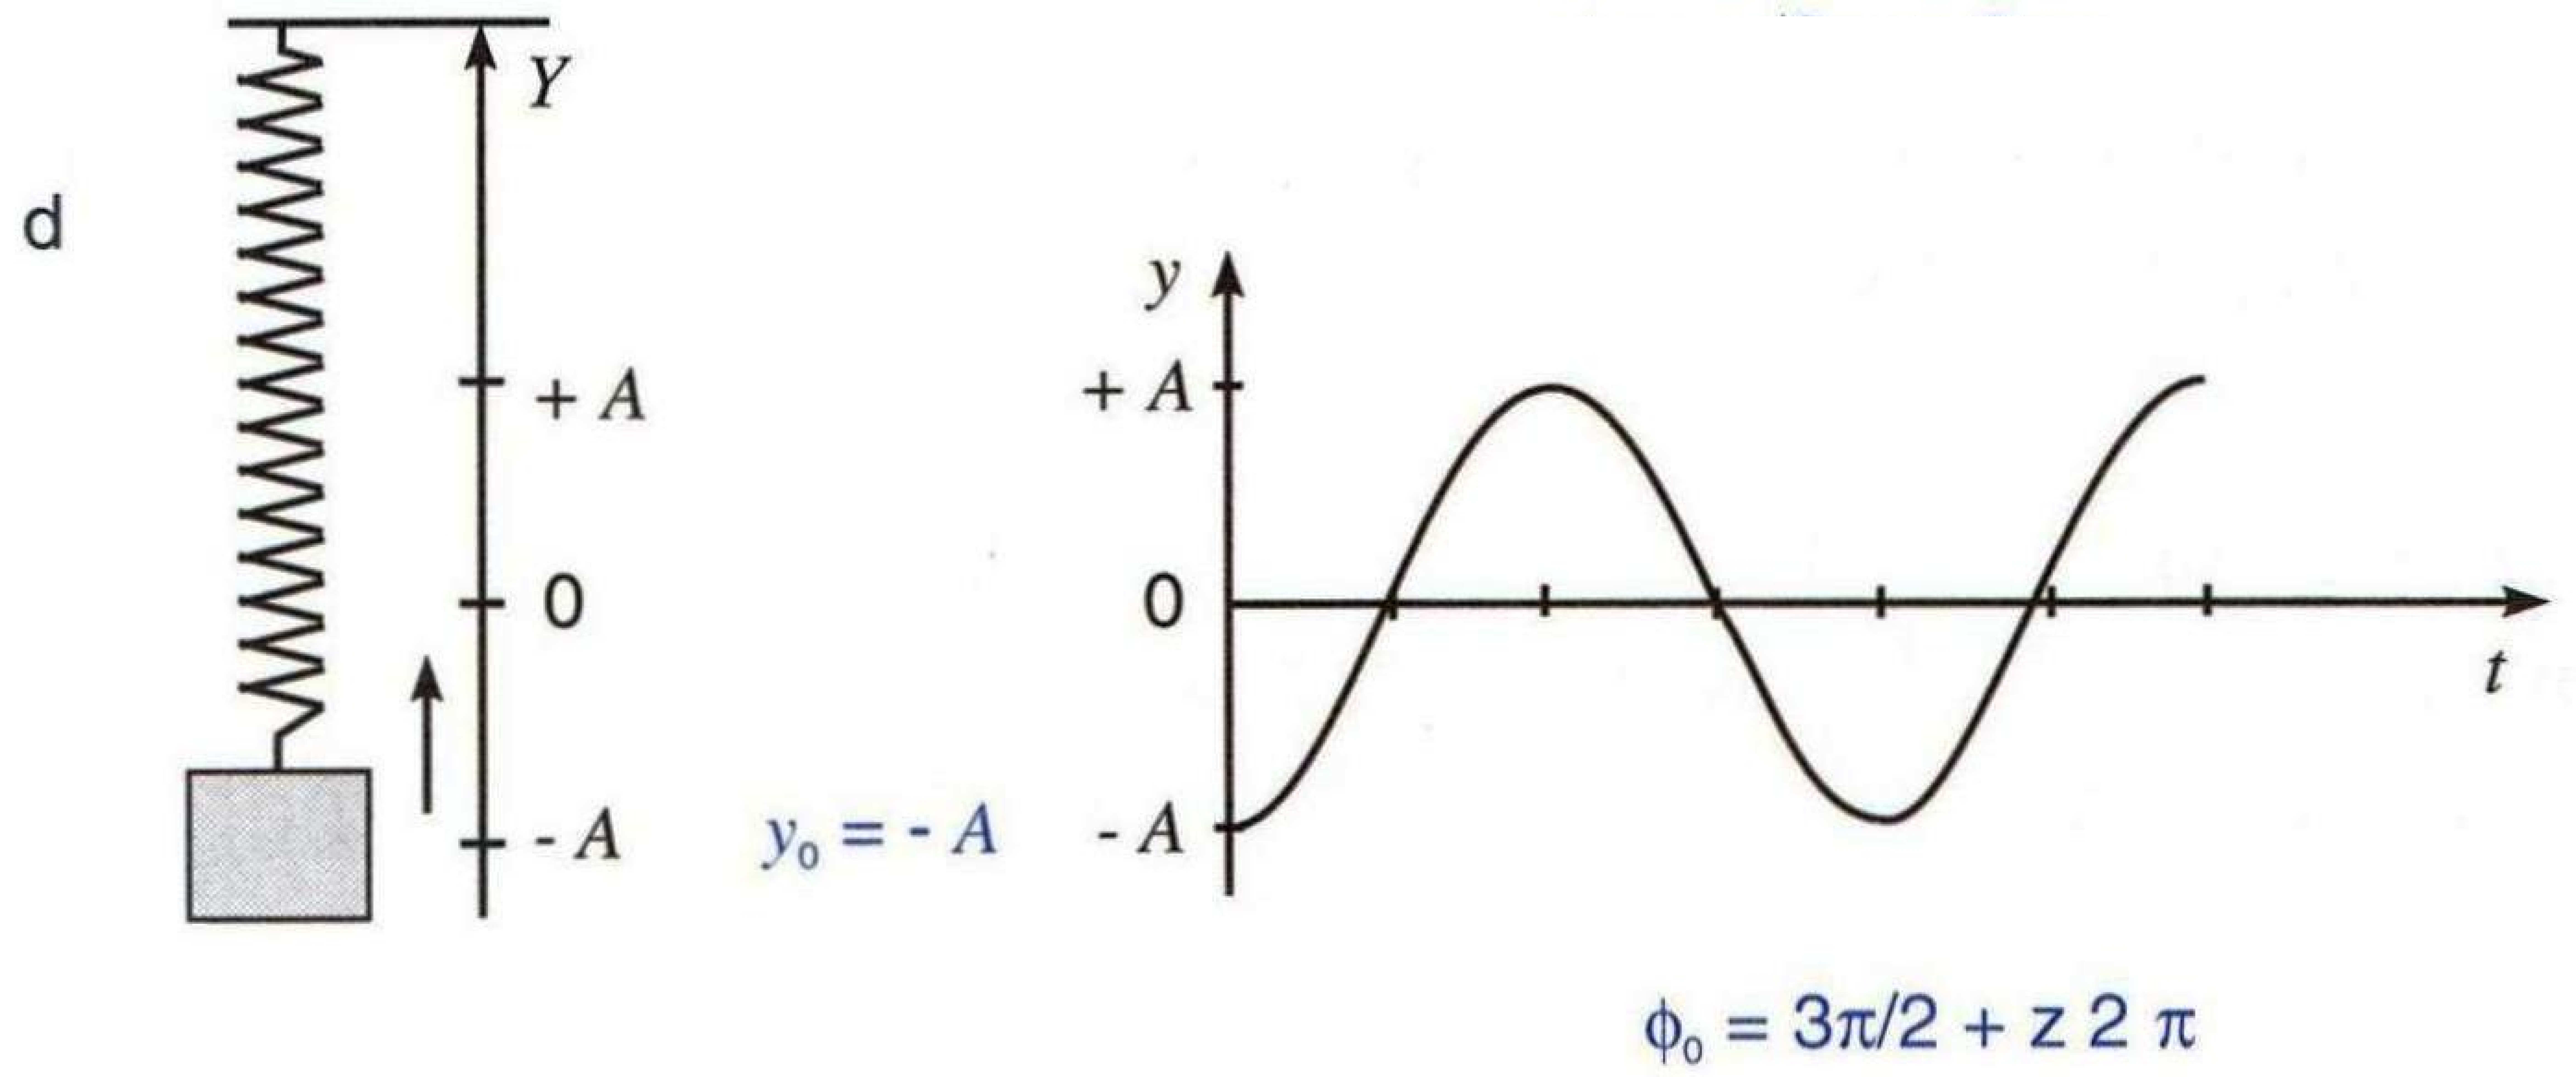
\includegraphics[width=.9\textwidth]{trillendeveer_d}
		
	\end{image}
	\captionof{figure}{Relatie tussen beginpositie en beginfase}
	
	\clearpage
	%%\newpage
	
	Naast in detail de beweging te hebben bestudeerd, kunnen we ook naar het energieverloop kijken. Hiertoe vullen we gewoonweg de positie en de snelheid in de formules voor energie in.
	\begin{eqnarray*}
	E_k&=&\frac{mv^2}{2}=\frac{1}{2}m\omega^2A^2\cos^2(\omega t+\varphi)\\
	E_p&=&\frac{1}{2}kx^2=\frac{1}{2}kA^2\sin^2(\omega t+\varphi)=\frac{1}{2}m\omega^2A^2\sin^2(\omega t+\varphi)
	\end{eqnarray*}
	Deze hangen duidelijk af van de tijd. Wanneer we naar de totale energie kijken, vinden we -- zoals we volgens de wet van behoud van energie mogen verwachten -- dat deze constant is.
	\begin{eqnarray*}
	E=E_k+E_p=\frac{1}{2}m\omega^2A^2\left(\sin^2(\omega t+\varphi)+\cos^2(\omega t+\varphi)\right)=\frac{1}{2}m\omega^2A^2
	\end{eqnarray*}
	\begin{image}
	
	%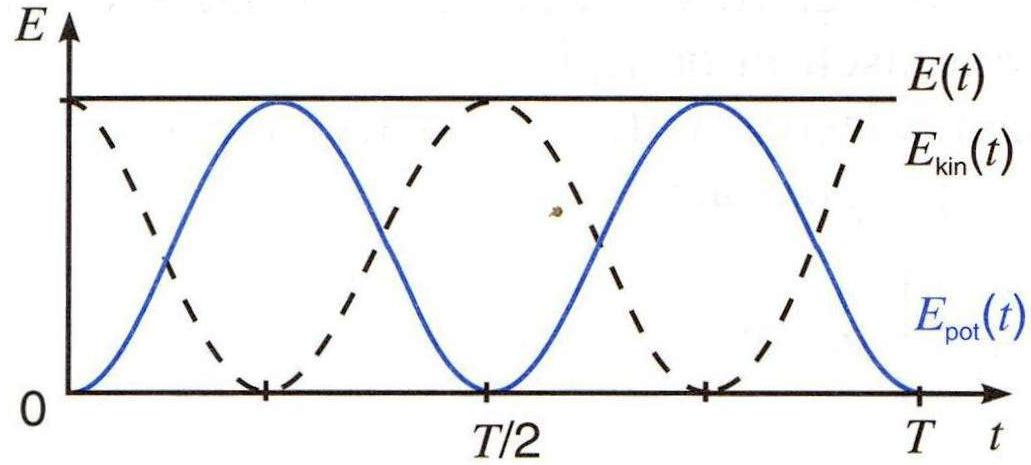
\includegraphics[width=.7\textwidth]{EpEkE}
	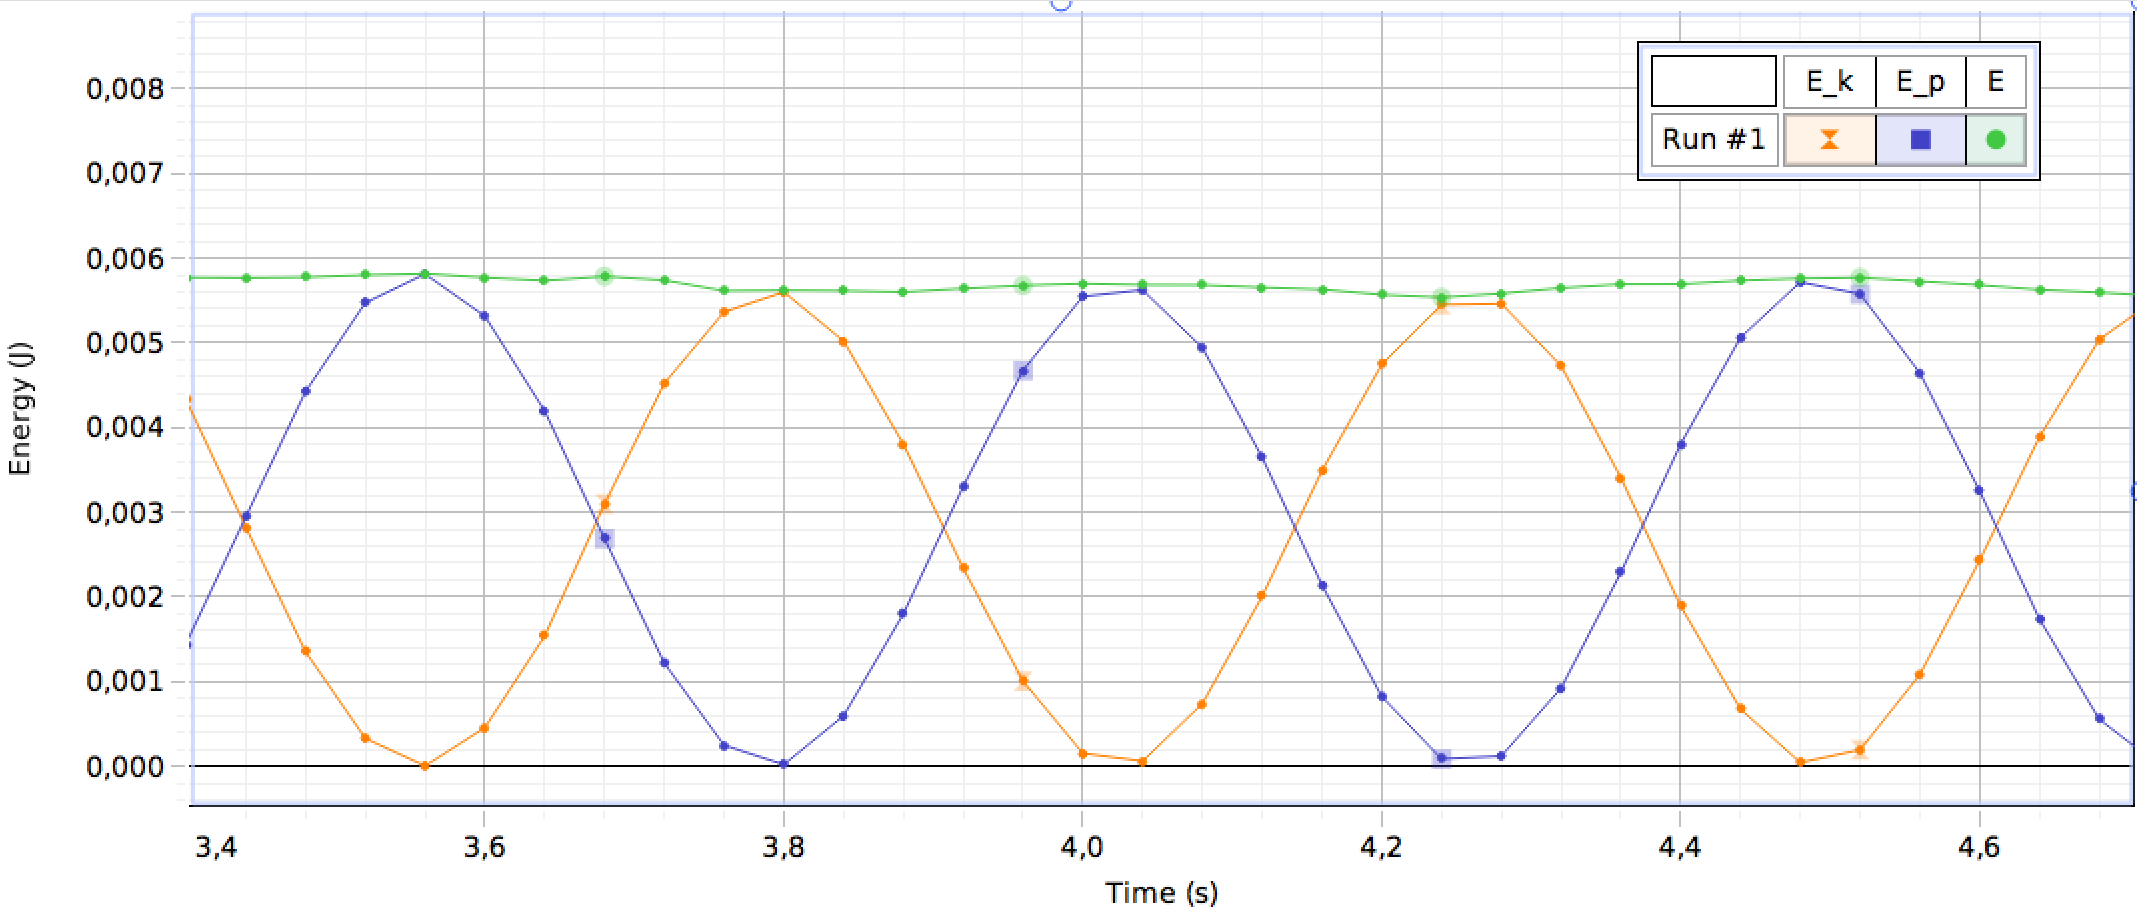
\includegraphics[width=.9\textwidth]{ht_behoud_energie}
	\end{image}
	Merk op dat de energie van een trilling recht evenredig is met het kwadraat van de amplitude. Een golf in de zee die dus twee keer zo hoog is, draagt vier keer zoveel energie met zich mee. In de figuur zie je mooi hoe de kinetische en de potentiële energie in elkaar worden omgezet; het verlies van de ene is de winst van de andere. Let op het verschil tussen de periode van de energievormen en de periode van de eigenlijke trilling \ldots
	
	%%%\newpage
	

\end{document}
